\documentclass[a4paper,12pt, english]{article}
\usepackage[T1]{fontenc}
\usepackage[utf8]{inputenc}
\usepackage{graphicx}
\usepackage{babel}
\usepackage{amsmath}
\usepackage{ulem}
\usepackage{a4wide}
\usepackage{graphicx}
\usepackage{listings}
\usepackage{tabularx}
\usepackage{tabulary}

\begin{document}

\begin{titlepage}
\begin{center}
\textsc{\Large Computational Physics, Project 3}\\[0.5cm]
\textsc{Vilde Eide Skingen and Kari Eriksen}\\[0.5cm]

\end{center}
\end{titlepage}

\begin{abstract}
The aim of project 3 is to create a code for simulating the solar system. In the first part we will look at a hypothetical solar system consisting of the Sun and the Earth. We will assume that the Sun's mass is sufficiently large, so that its motion can be neglected. With this assumption we will compute the motion of the Earth using the Runge-Kutta solver to solve an ordinary differential equations. Later we will add several other planets to our simulation, and see how the forces between the objects effects the individual orbits.
What we find out is that the Runge-Kutta solver is not as stable for every timestep. Also there is a fine line between a to big initial velocity and a to small one. 

\end{abstract}

\section*{A model for the solar system}

\subsection*{Introduction}
In the first part of the project our goal is to calculate the position of Earth as a function of time. The only force in the project is the gravitational force between the heavenly bodies. We first look at a hypothetical solar system consisting only of the Earth and the Sun. However, we will write our program in such a way that it is easy to add other planets in our simulation. 

\subsection*{Theory}

In the first part of the project we will look at a hypothetical solar system with only one planet, the Earth, in orbit around the Sun. The only force in this problem is gravity, given by Newton's law of gravitation $$ F_G = \frac{GM_{sun}M_{Earth}}{r^2} $$
where $M_{sun}$ and $M_{Earth}$ are the masses of the Sun and Earth, $r$ the distance between them, and $G$ the gravitational constant. If we assume that the Sun has a much larger mass than the mass of the Earth, we can safely neglect the motion of the sun in the calculations. 

We will also assume that the orbit of Earth around the Sun is co-planar, and that it lies in the $xy$-plane. We  then get the following equations from Newton's second law of motion
$$\frac{d^2x}{dt^2} = \frac{F_{G,x}}{M_{Earth}}$$
$$\frac{d^2y}{dt^2} = \frac{F_{G,y}}{M_{Earth}}$$
where $F_{G,x}$ and $F_{G,y}$ are the $x$ and $y$ component of the gravitational force. 


\begin{figure}[h!]
  \centering
    	  \includegraphics[scale=0.4]{project3.png}
  \caption{\textit{Coordinate system with the Sun at the center and Earth located at (x,y) in orbit around the Sun}}
\end{figure}


From figure 1 we have that

$$F_{G,x} = - F_G  \hspace{0.7 mm} cos \theta = - \frac{GM_{sun}M_{Earth}}{r^2} \hspace{0.7 mm} cos \theta $$
$$F_{G,y} = - F_G \hspace{0.7 mm} sin \theta = - \frac{GM_{sun}M_{Earth}}{r^2} \hspace{0.7 mm} sin \theta $$


\begin{figure}[h!]
  \centering
    \includegraphics[scale=0.2]{project3_1.png}
  \caption{\textit{Relation between the distance between Earth and the Sun and the angle $\theta$}}
\end{figure}

and figure 2 gives that

$$ cos \theta = \frac{x_i}{r} $$
$$ sin \theta = \frac{y_i}{r} $$

We can rewrite the second-order ordinary differential equations as a set of coupled first order differential equations. 
We know that the velocity is connected to the position by the time derivative so that \\
$$ \frac{dx}{dt} = v_x \hspace{20 mm} \frac{dy}{dt} = v_y$$
and thus we have that \\

$$ \frac{dv_x}{dt} = \frac{F_{G,x}}{M_{Earth}} \hspace{20 mm} \frac{dv_y}{dt} = \frac{F_{G,y}}{M_{Earth}} $$
\\

These ordinary differential equations can be solved by numerical methods. However, before doing so, we should find a suitable choice of units. We choose to use the astronomical units in our project. The astronomical unit of length is given to be the average distance between the Sun and the Earth, $1 AU = 1.5*10^{11} m$. It is convenient to measure time in years, since this better suits the cycles of the solar system. We choose to measure mass relative to the Sun's mass.

In preparation of constructing a computational solution, we convert the equations of motion into a discretized set of equations. The acceleration is given by Newton's second law, $$ F = ma.$$ The change in velocity is $a \Delta t$, and the change in position is $v \Delta t$. Thus we find the q
equations for the Earth effected by the gravitational force from the Sun to be
\\

$$v_{x,i+1} = v_{x,i} - \frac{G M_{sun} x_i}{r_i ^3} \hspace{0.5mm} \Delta t $$ 

$$x_{i+1} = x_i + v_{x,i+1} \Delta t $$

$$v_{y,i+1} = v_{y,i} - \frac{G M_{sun} y_i}{r_i ^3} \Delta t $$

$$y_{i+1} = y_i + v_{y,i+1} \Delta t $$
\\

where $\Delta t$ is the time step. In the case of circular orbit we have that $4 \pi ^2 = GM_{sun}$.

For circular motion we know that the force must obey the following relation \\
$$\frac{M_{Earth}v^2}{r} = F_G = \frac{GM_{sun}M_{Earth}}{r^2}$$ where $v$ is the velocity of the Earth. 
For circular orbit the velocity of the Earth is $v = \frac{2 \pi r}{1 year}$, where the distance between Sun and Earth is $r = 1 AU$. Hence $v = 2 \pi (AU/years)$. Rearranging the equation we find\\
$$v^2r = GM_{sun} = 4 \pi ^2 AU^3/years^2$$
\\
For circular motion the velocity will be tangential. It follows that if we choose the initial conditions $ x = 1 AU $ and $ y = 0$, with velocities $v_x = 0$ and $v_y = v_{tangential} = 2 \pi AU/year$ we will get a circular orbit.  


\subsection*{Method}
To compute the trajectories of the different astronomical objects we made a vector $A$ that holds information of the initial position and velocity in x and y direction for all objects. That is our vector $A$ is a $4*n$ vector, where $n$ is the number of objects.

\[ A = \left( \begin{array}{c}
x - object 1\\
y - object 1\\
vx - object 1\\
vy -object 1\\
x - object 2\\
... \\
vy - object n \end{array} \right)\]   

We computed the time derivative of this vector and saved it in a vector $dAdt$. The derivative of the position equals the velocity, so these values we could read directly from our $A$ vector. 
To find the acceleration, the time derivative of the velocities, we computed the radius between the different objects, and calculated the force between them. By using Newton's second law we found the acceleration of each object. We then used these values in the Runge-Kutta 4 scheme to make estimates of the next positions and velocities. For each time step we wrote the $x$ and $y$ values to a file so that we could make plots of the objects trajectories.    

The Runge-Kutta solver is a method for solving ordinary differential equations for which we know the initial values. In this project the motion of the planets are described by a second-order differential equation of the position as a function of time. We want to find the propagation of this function forward in time starting from the given initial values. 

Taylor series expansion of a function $x$ around $t$ gives
$$ x(t+ \Delta t) = x(t) + \frac{dx}{dt} \Delta t + \frac{1}{2} + \frac{d^2 x}{d^2 t} (\Delta t)^2 + \cdots $$

If we assume a reasonable smooth function $x(t)$ and a small interval $\Delta t$ we can approximate $x(t)$ to $x(t + \Delta t)$ as long as we know the derivatives of $x(t)$. 
When using the Runge-Kutta approximation one estimates the slopes at four points, once at the initial point, twice at the trial midpoint and once at the trial endpoint. 
$$ k_1 = \Delta t f(t_i,x_i) \\
k_2 = \Delta t f(t_i + \Delta t /2, x_i + k_1/2) \\
k_3 = \Delta t f(t_i + \Delta t/2, x_i + k_2/2) \\
k_4 = \Delta t f(t_i + \Delta t, x_i + k3) $$

These four derivatives constitute the next value in our propagation
$$x_{i+1} = x_i + \frac{1}{6} (k_1 + 2(k_2+k_3) + k_4$$ 

For the Runge-Kutta 4 scheme the local error in the approximation is $O([\Delta t]^3)$. \\

To check the stability of our program for different time steps $\Delta t$ we made a program that runs over various values of $\Delta t$ and picks out the maximum radius in the Earth's orbit around the Sun. Giving the initial values for circular orbit this radius should yield $1 AU$. We wrote the $\Delta t$ values with the corresponding maximal radius to a file, and made a plot of this. \\

In the case of circular orbit we also wanted to check that the kinetic and potential energy and the angular momentum are constants, as they should be. We then wrote functions which took in the needed values for the position, velocity and radius to compute the three wanted values. For each step in our propagation for the trajectories we printed these values to a file.\\  

We also want to check how Jupiter effects the earth with it's gravitational field. 
As in the previous cases, there are some new values we wish to save. First we made a plot of the differance between the x-coordinates and the y-cordinates, for when the sun was the only object infuencing the earth, and when jupiter influences as well. Then we already had the needed values. But to see how the earth moves differentely in the different cases, we made a plot of the distance between Earth and origo. Instead of using $r$, we calculated new values, $L = \sqrt{x_i^2 + y_i^2},$ which is the distance between Earth and origo. 
These we wrote to two new files, $distance\_from\_sun\_1.dat$ and $distance\_from\_sun\_2.dat.$ \\

Finally we wanted to plot the solar system with all the planets. Having written the program in the idea of making it easy to impliment other objects, this was straight forward. But in order to impliment the objects, we need the initial conditions, like position and velocity. The masses of the different planets, we find in the project sheets. These we converted into solar masses, just a bit easier to use. Positioning of all the planets we did searching on Wolfram Alpha. This gave us the distance between the sun and all the respective planets.  
And finally we found the velocity from a webpage \url{http://nssdc.gsfc.nasa.gov/planetary/factsheet/}.\\

Here we used the orbital velocity and transformed these relative to Earths velocity ($2\pi$), in $1/AU.$ 
How to place all the planets around the sun, we did in the simplest way. We put them all on a line on the x-axis, with initial velocity in y-direction. \\

Later we want to keep the center of mass in our solar system fixed. When we have a three-body problem, we give the sun a push in the other direction of Jupiter and Earth, which matches their combined speed. This keeps the total momentum zero. In this case this would give
$$p = M_{\odot}v_0.$$
With 
$$M_{\odot} = 1$$ 
we get 
$$p = M_{earth}v_0 + M_{jupiter}v_0$$
$$p = 0.0026585.$$   
Since the momentum should point in the opposite direction of Jupiters and Earths, the initial velocity of the sun would become $v_0 = -0.0026585.$ 


\begin{table} [h!]
\caption{Important facts about our planetary system}
\centering
\begin{tabular}{l | l l l} 
\hline
Object & $r_0$ [AU] & $v_0$ [1/AU] & M [$M_{\odot}$]\\
\hline
Earth & 1.0 & $2\pi$ & 3.0e-6  \\ [0.5ex]
Sun & 0.0 & 0.0 & 1.0 \\
Venus & 0.727 & 7.385 & 2.45e-6 \\
Mercury & 0.354 & 10.107 & 1.66e-7 \\
Mars & 1.642 & 5.085 & 3.23e-7 \\
Jupiter & 5.168 & 2.764 & 9.55e-4 \\
Saturn & 9.883 & 2.047 & 2.86e-4 \\
Uranus  & 20.06 & 1.435 & 4.36e-5 \\
Neptune & 30.04 & 1.139 & 5.17e-5 \\
Pluto & 32.36 & 0.992 & 6.61e-9 
\end{tabular}
\end{table}


\subsection*{Results}
When running our program for the two-body system of the Earth and the Sun and for the initial values we in theory predicted to be circular we found that our program lives up to our expectations. Figure 3 shows the plot we got of the Earth's orbit around the Sun with the initial values for circular motion.

\begin{figure}[h!]
  \centering
    \includegraphics[scale=0.5]{circular_orbit_earth.png}
  \caption{\textit{Circular orbit of the Earth only effected by the gravitational force from the Sun}}
\end{figure}


When increasing the initial velocity the orbit will be elliptical, until we reach a high enough velocity for the Earth to escape it's orbit around the Sun. In figure 4 we see the elliptical orbit when using an initial velocity of $v = 2 \pi +1$. In figure 5 the initial velocity is increased to $v = 2 \pi + 2.3$, and we see that this is to great a speed for the gravitational force to keep the Earth in orbit. Hence, the Earth escapes the gravitational field of the Sun and continues to infinity.  

\begin{figure}[h!]
  \centering
    	\includegraphics[scale=0.5]{circular_orbit_1.png}
  \caption{\textit{Orbit of the Earth with a initial velocity of $v = 2 \pi +1$}}
\end{figure}

\begin{figure}[h!]
  \centering
    \includegraphics[scale=0.5]{circular_orbit_2.png}
  \caption{\textit{Trajectory of the Earth with a initial velocity large enough to escape the gravitation field from the Sun}}
\end{figure}


An initial velocity close to, but less, than the initial velocity of circular orbit will, give elliptical orbit. However, if we decrease the velocity by a certain amount, the Earth will be dragged in elliptical spirals towards the Sun. The speed of which the Earth spirals towards the Sun will depend on the magnitude we decrease the initial velocity. If we run our program for a time limit so that the Earth gets very close to the Sun, the forces working on Earth will get to big for our program to handle. We will get a case of overflow, and thus it looks like the Earth is sent out from the Sun and escapes the gravitational force working on it (as seen in figure 6).   
     
\begin{figure}[h!]
  \centering
    \includegraphics[scale=0.5]{circular_orbit_3.png}
  \caption{\textit{The low initial velocity causes the Earth to be dragged towards the Sun. When it gets close to the Sun it is sent out from the gravitational field}}
\end{figure}


When running for different time steps we found that our algorithm highly depends on the choice of step. For instance, when looking at the initial velocity that should give us circular motion, the program will not yield the wanted result if we do not choose the right time step. Here, in figure 7, for $N = 20, t_f = 2$ and the initial conditions that should yield circular motion.
  
\begin{figure}[h!]
  \centering
   	 \includegraphics[scale=0.5]{timesteps_circular.png}
  \caption{\textit{Unstable algorithm for large time step}}
\end{figure}

From figure 8 and 9 we see the maximal radius in our orbit for different choice of $\Delta t$. The analytical value for the radius is the distance at circular orbit, $1 AU$. We see that the algorithm is very unstable for too large time steps.

\begin{figure}[h!]
  \centering
   	 \includegraphics[scale=0.5]{timesteps_stability.png}
  \caption{\textit{Plot over various time steps and the maximal radius}}
\end{figure}
 
\begin{figure}[h!]
  \centering
   	 \includegraphics[scale=0.5]{timestep_stability3.png}
  \caption{\textit{Plot over various time steps and the maximal radius}}
\end{figure}

\begin{figure}[h!]
  \centering
   	 \includegraphics[scale=0.5]{timesteps_stability2.png}
  \caption{\textit{Unstable algorithm for too large time step}}
\end{figure}



\begin{figure}[h!]
  \centering
   	 \includegraphics[scale=0.4]{energi.png}
  \caption{\textit{List of kinetic and potential energy and angular momentum for different time steps}}
\end{figure}

In the case of circular orbit we wanted to test that the kinetic and potential energy and the angular momentum are constants. Printing out the values for these three quantities we found that they all were constants, as they should be.\\

Studying the case of Jupiters effect on Earth, there are number of ways of showing how Jupiters gravitational field pulls on Earth. We have both made plots of Earths motion, and the distance between Earth and origo. Because the distance between the earth and the Sun does not change when we add Jupiter as a third object,because the Sun moves as it is effected by Jupiter as well, we need to plot the distance from origo instead. \\

When we plot Earths orbit around the Sun in the first case, that is Earth is only influenced by the Sun, we see that the orbit is almost sircular. But the radius of Earths distance from the Sun, increases for every year. In the second case, that is adding Jupiter as a third object, we can see very clearly that the orbit is effected by something. And this something is Jupiters gravitation. \\

If we now try to plot the distance between Earth and origo, we can more easily see how Earths motion is effected by Jupiter. \\

When the Sun is the only object influencing Earths motion, we can see that the radius increases by every year. But when Jupiter is implemented, the radius oscillates around the red line. In reality, the mass center is not in the center of the Sun, as we have used up til this moment. If we implement a fixed mass center, for our three-body problem, we see from figure 15 that the orbit of the Earth again is as for the two-body problem (Sun - Earth). \\

If we try to increase Jupiters mass by a factor of 10 and 1000, we get plots like the ones we have in figure 16. \\

As a last assignment we plot the entire solar system. \\

\begin{figure}[h!]
  \centering
   	 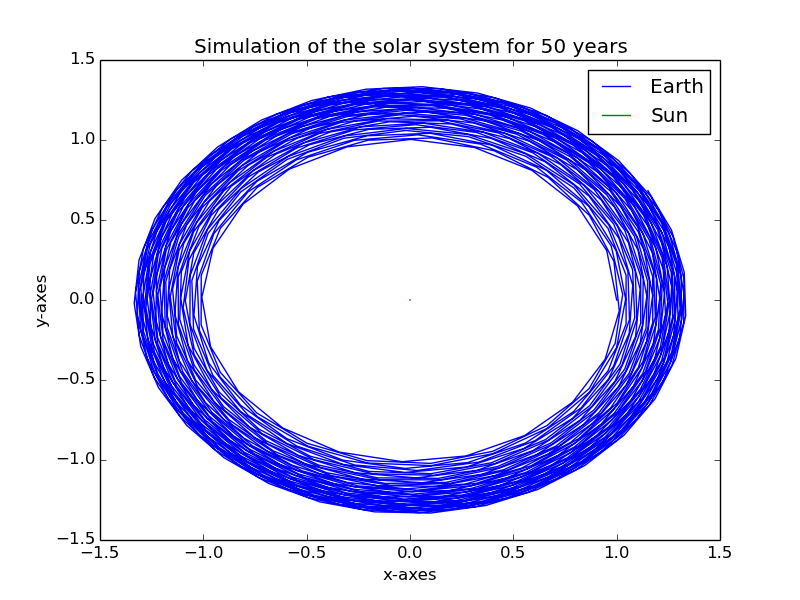
\includegraphics[scale=0.4]{Sun_earth.png}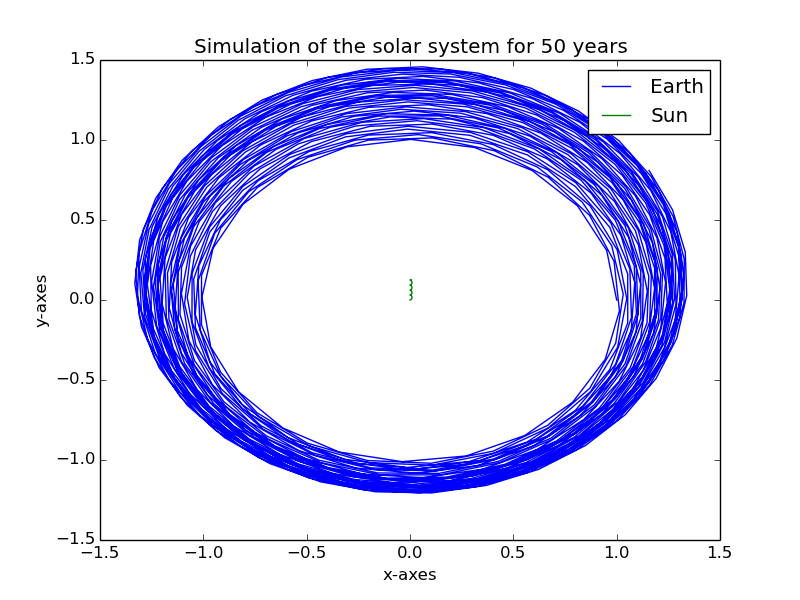
\includegraphics[scale=0.4]{Earth_sun_jupiter.png}
  \caption{\textit{The first plot shows Earths orbit, when it is only effected by the Sun. The second one is of when Jupiter is inplemented in our simulation.}}
\end{figure}


\begin{figure}[h!]
  \centering
   	 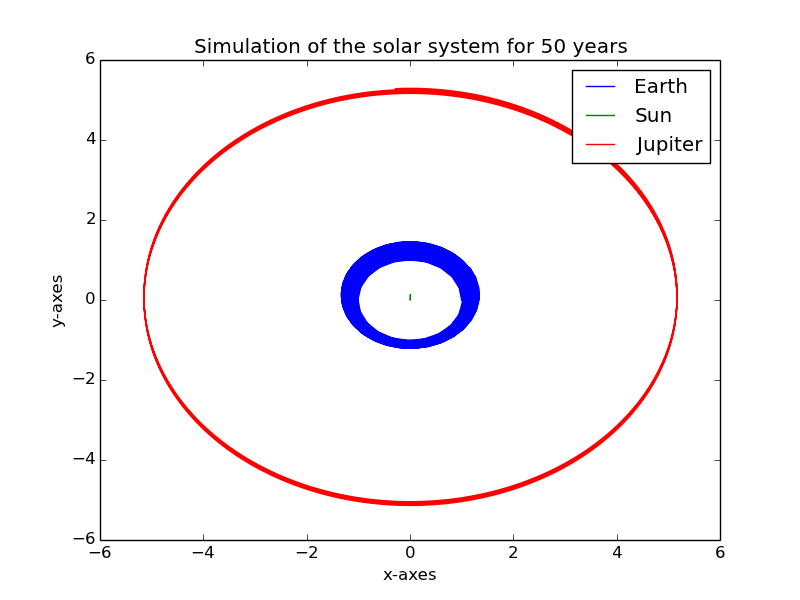
\includegraphics[scale=0.5]{Sun_earth_jupiter.png}
  \caption{\textit{Here we can see Jupiters orbit around the Sun.}}
\end{figure}




\begin{figure}[h!]
  \centering
   	 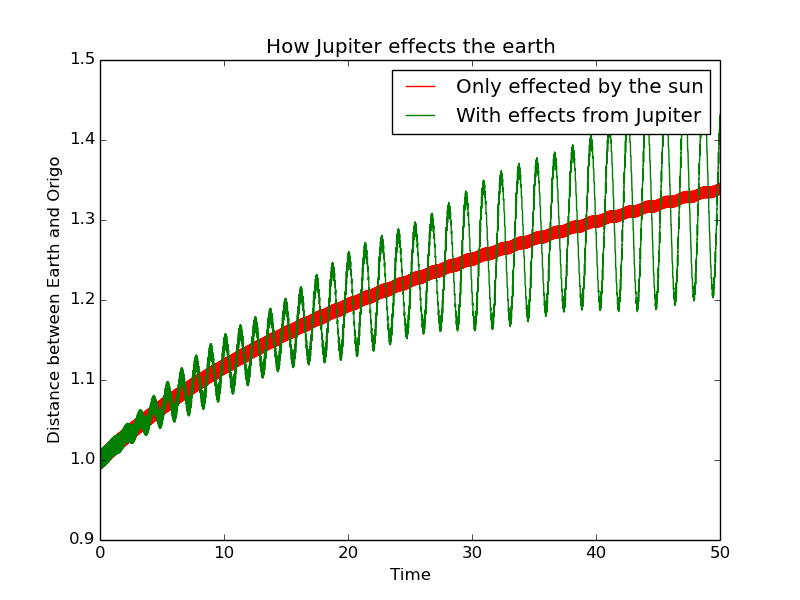
\includegraphics[scale=0.5]{Effect_of_Jupiter.png}
  \caption{\textit{}}
\end{figure}


\begin{figure}[h!]
  \centering
   	 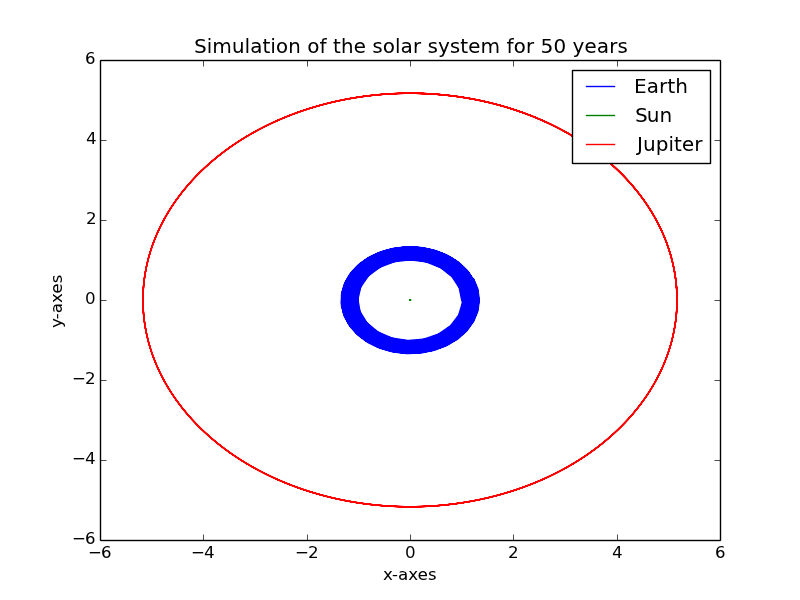
\includegraphics[scale=0.5]{Mass_center_Jupiter.png}
  \caption{\textit{This looks just like the one for our two-body problem, of only the Sun and Earth. Now the mass center is fixed, and Earths orbit is stable again.}}
\end{figure}



\begin{figure}[h!]
  \centering
   	 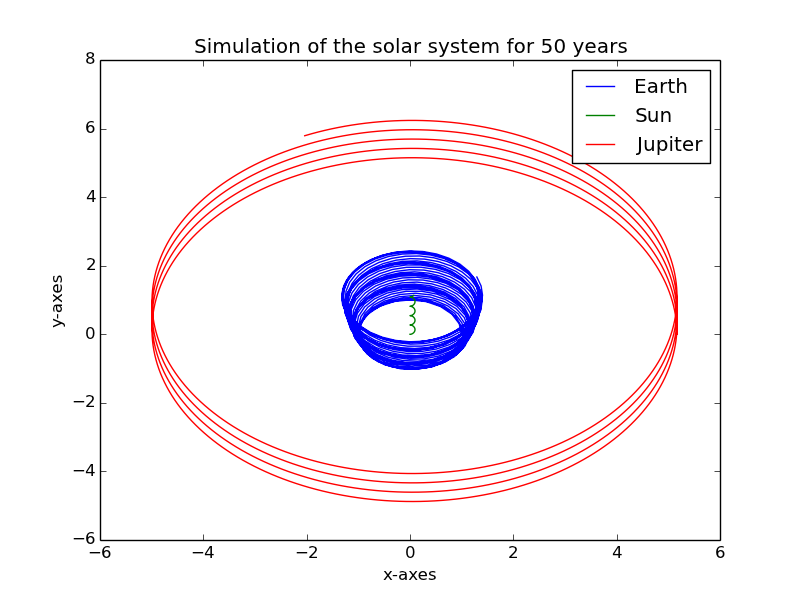
\includegraphics[scale=0.4]{Jupiter_10.png}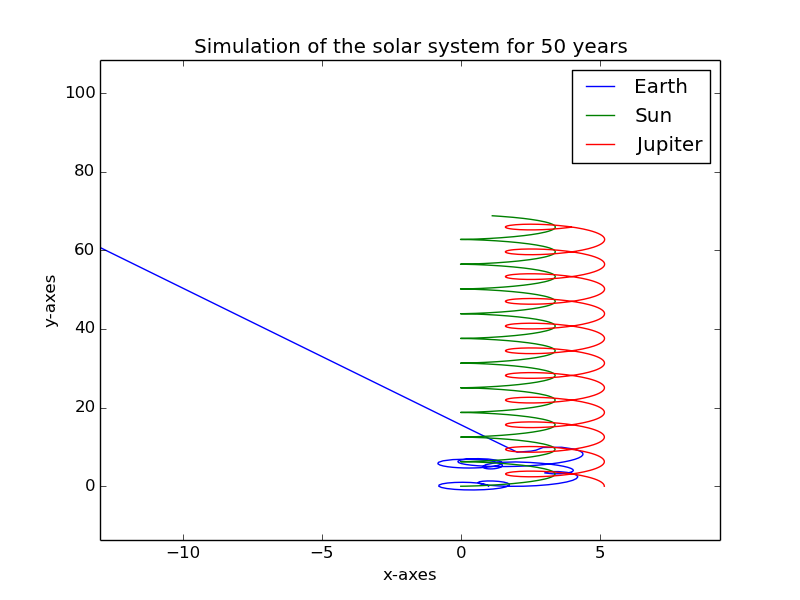
\includegraphics[scale=0.4]{Jupiter_1000.png}
  \caption{\textit{Here we see how Earth is effected when we increase the mass of Jupiter by factors of 10 and 1000, respectevly.}}
\end{figure}


\begin{figure}[h!]
  \centering
   	 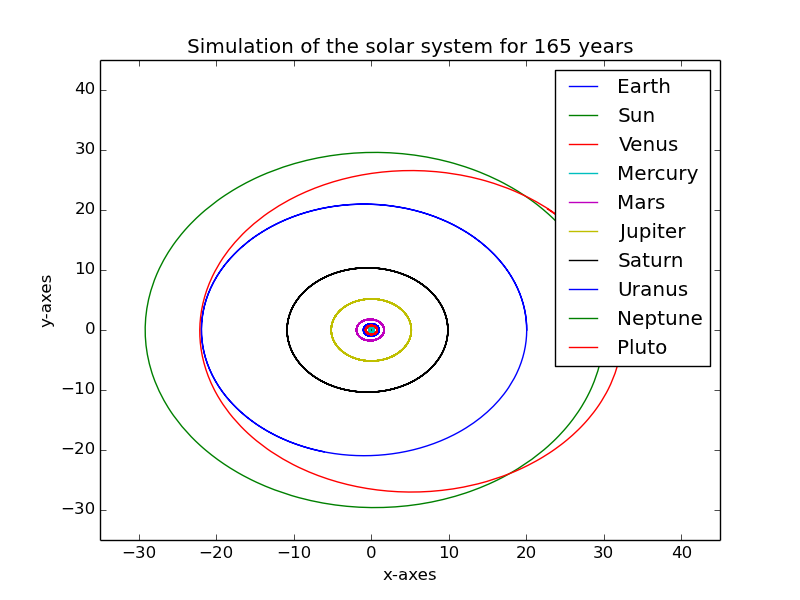
\includegraphics[scale=0.4]{Solar_system.png}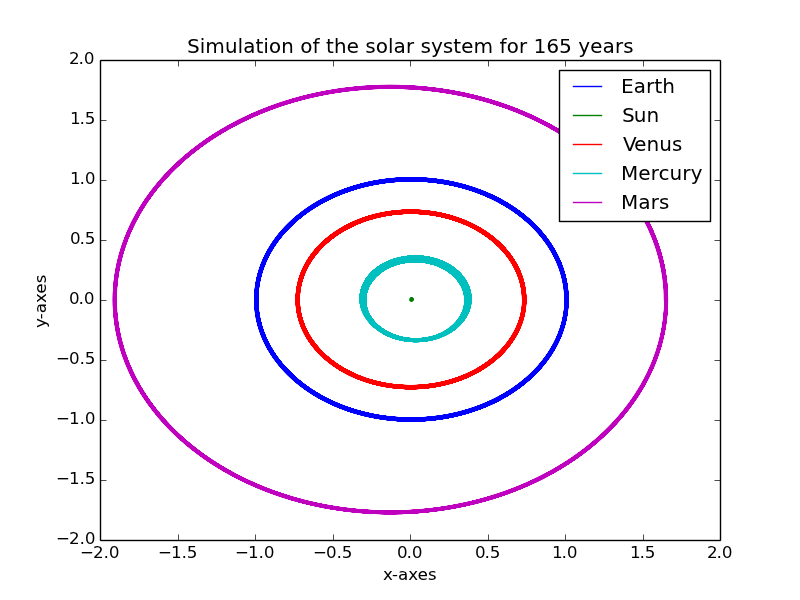
\includegraphics[scale=0.4]{Solar_system_4planets.png}
  \caption{\textit{The entire solar system, with all the eight planets and Pluto! And a closer zoom on the four first planets.}}
\end{figure}



\begin{figure}[h!]
  \centering
   	 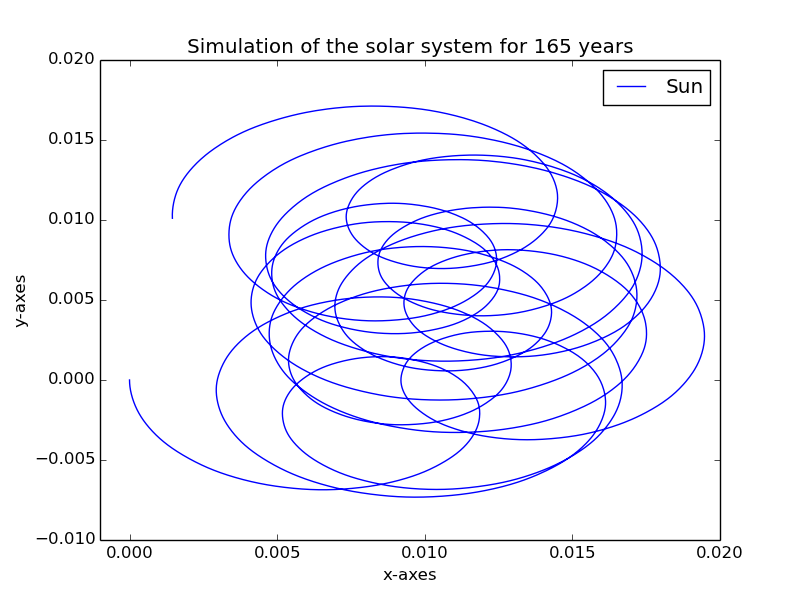
\includegraphics[scale=0.5]{Solar_system_sun.png}
  \caption{\textit{Here we see the motions of the Sun. It orbits around it self}}
\end{figure}


\subsection{Conclusion}

We have seen during this project that the solver we have used to solve the differential equations is quite unstable for the wrong choice of time step, $\Delta t$, and highly dependent of the given initial values. Smaller values of $\Delta t$ gives smaller errors (if we ignore the possibility of round-off errors), but reducing $\delta t$ also leads to a greater computational cost. However, our program was not very time consuming, so this is a cost we could live with in this case. The stability of our solver will also depend on how slowly or fast the function to integrate varies. In the case of great variance our approximation will not be very good. One strategy is to decrease the step size, and thus get a interval with less variance. This, again, leads to more cycles and may lead to loss of numerical precision. An alternative could be to use higher-order RK methods, where you evaluate the slope at more points. This leads again to more cycles, and there is no guarantee for an improved error.  \\

From figure 12 in the second picture, Jupiters effect on Earth is clear. But how big the effect is, we can see better in figure 14. The radius oscillates around the red line. So the effect is changing from big to small, what looks like every year. From figure 13 we can maybe get an understanding. When Jupiter is north of the Sun, the pull is bigger, but decreases more and more as it moves south. This is because the Sun moves north. As Jupiter gets closer to the south, the pull from the Sun decreases, and Jupiter will get a bigger radius in this direction. Therefore the pull on Earth, from Jupiter, gets smaller, and the radius of the Earth get smaller. But this is all because the Sun moves north. Way this is, may be because we give the planets a velocity in this direction, and the Sun gets effected by this. \\

As mentioned before, we should really fix our center of mass. If we do this, meaning we change suns initial velocity from 0 to -0.0026585, we see in figure 15 how the entire system stabilizes. 
If we change Jupiters mass by a factor of 10 and 1000 we get the plots in figure 16. If we first look at the plot where we have increased Jupiters mass by a facto 10, it is obvious that the pull from Jupiter is greater, as the Sun also moves much more than in the previous case. But an increase by 1000, it is even more obvious how Jupiter almost dominates the system. Now the mass of Jupiter is almost as big as the Sun, 0.955 $M_{\odot}$. The Earths velocity is way to small, and the size as well, compared to the other objects and gets sent out of the gravitational field. This is as mentionaed before, a case of overflow. Jupiter and the Sun will pull on one another, and just circulate in each others gravitational field.\\

 Finally we put in all the other planets, and the plots can be seen figure 17. The first plot shows all the planets. It is close to the real case, all the planets are close to co-planar and orbits almost circular. Exept for Pluto. Plutos orbit should be an elongated ellipse. Unfortunately is was a bit difficult to place Pluto in the system, so it would get this orbit. We used the planets current position at that day (Okt. 25.), which is almost the same as Neptune. Its position and initial velocity was perhaps not coherent. It would therefore not take the orbit it should. Otherwise the simulated solar system is close to the real case.\\ 

At last we look at figure 18. This plot shows the motion of the Sun, as all the planets are included. It looks as though the Sun is much more stable, circulating around itself, as we implement more objects and of course have a fixed mass center.  
If we increase the mass around the Sun, it will pull a bit in every direction, as the planets have different orbital periodes. It will keep itself in the center of the system. 
 

\end{document}    
